%  --------------------------------------------------------------------------
%  Bachelorarbeit IT Qualitätsmanagement für Webprojekte
%  Created by Marc Egli on 2013-01-25.
%  --------------------------------------------------------------------------

%  --------------------------------------------------------------------------
%  Latex Document Settings
%  --------------------------------------------------------------------------
\documentclass[
11pt, % Schriftgrösse
a4paper, % A4 Papier
BCOR10mm, % Absoluter Wert der Bindekorrektur, z.B. BCOR1cm
DIV14, % Satzspiegel festlegen siehe
       % http://www.ctex.org/documents/packages/nonstd/koma-script.pdf
footsepline = false, % Trennlinie zwischen Textkörper und Fußzeile
                     % bei normalen Seiten
headsepline, % Trennlinie zwischen Kopfzeile und Textkörper
             % bei normalen Seiten
oneside, % Zweiseitig
openright,
halfparskip, % Europäischer Satz mit Abstand zwischen den Absätzen
abstracton, % inkl. Abstract
listof=totocnumbered, % Abb.- und Tab.verzeichnis im Inhaltsverzeichnis
bibliography=totocnumbered % Lit.zeichnis in Inhaltsverzeichnis aufnehmen
]{scrreprt}

\usepackage[automark]{scrpage2} % Gestaltung von kopf- und Fußzeile
\usepackage[ngerman]{babel}
\usepackage[ngerman]{translator}
\usepackage{tocbasic}
\usepackage[utf8]{inputenc}
\usepackage{lmodern} % Latin Modern
\usepackage[T1]{fontenc}
\usepackage{hyphenat}
\usepackage{ae} % Schöne Schriften für PDF-Dateien
\usepackage{multirow} % tabellenzellen zusammenfassen
\usepackage{float}

% Tradmark
\def\TTra{\textsuperscript{\texttrademark}}

%1.5 Zeilenabstand
\usepackage[onehalfspacing]{setspace}

% Festlegung des Seitenstils (scrpage2)
\pagestyle{scrheadings}
\clearscrheadfoot
\automark[]{chapter}

% \lehead{\sffamily\upshape\headmark}
% \cehead{}
% \rehead{}
% \lefoot[\pagemark]{\upshape \pagemark}
% \cefoot{}
% \refoot{}
% \lohead{}
% \cohead{}
\lohead{\sffamily\upshape\headmark}
\lofoot{}
\cofoot{}
\rofoot[\pagemark]{\scshape \pagemark}

% Surround parts of graphics with box
\usepackage{boxedminipage}

% Package for including code in the document
\usepackage{listings}

% If you want to generate a toc for each chapter (use with book)
\usepackage{minitoc}
\usepackage{longtable}

% Abkürzungsverzeichnis erstellen.
\usepackage[printonlyused]{acronym}

% schöne Tabelle zeichnen
\usepackage{booktabs}
\renewcommand{\arraystretch}{1.4} %Die Zeilenabstände in Tabllen angepasst.

% für variable Breiten
\usepackage{tabularx}

% Durchgestrichener Text
\usepackage[normalem]{ulem} %emphasize weiterhin kursiv

% This is now the recommended way for checking for PDFLaTeX:
\usepackage{ifpdf}

\usepackage{eurosym}

\usepackage{natbib}

\usepackage{paralist}

\usepackage{array,ragged2e}

% glossary
\usepackage[toc, numberedsection, acronym, numberline, nonumberlist]{glossaries}

\usepackage[]{hyperref}
\hypersetup{
  bookmarks=true,         % show bookmarks bar?
  unicode=true,           % non-Latin characters in Acrobat’s bookmarks
  pdftoolbar=true,        % show Acrobat’s toolbar?
  pdfmenubar=true,        % show Acrobat’s menu?
  pdffitwindow=true,      % window fit to page when opened
  pdfstartview={FitH},    % fits the width of the page to the window
  pdftitle={Semesterarbeit},   
  pdfauthor={Marc Egli},
  pdfsubject={IT Qualitätsmanagement für Webprojekte},
  pdfcreator={TeX Live 2013},
  pdfproducer={pdfTeX 3.1415926-2.4-1.40.13},
  pdfnewwindow=true,      % links in new window
  colorlinks=true,       % false: boxed links; true: colored links
  % linkcolor=blue,          % color of internal links
  % citecolor=black,        % color of links to bibliography
  % filecolor=magenta,      % color of file links
  % urlcolor=cyan          % color of external links
  linkcolor=black,          % color of internal links
  citecolor=black,        % color of links to bibliography
  filecolor=black,      % color of file links
  urlcolor=black,          % color of external links
}

\ifpdf
    \usepackage[pdftex]{graphicx}
\else
    \usepackage{graphicx}
\fi
\pagenumbering{Alph}
\makeatletter 
\let\orgdescriptionlabel\descriptionlabel 
\renewcommand*{\descriptionlabel}[1]{% 
  \let\orglabel\label 
  \let\label\@gobble 
  \phantomsection 
  \edef\@currentlabel{#1}% 
  %\edef\@currentlabelname{#1}% 
  \let\label\orglabel 
  \orgdescriptionlabel{#1}% 
} 
\makeatother 

\makeglossaries
%!TEX root = index.tex
\newglossaryentry{Content Management System}
{
  name={Content Management System},
  description={Content Management System}
}

\newglossaryentry{unittest}
{
  name=Unittest,
  plural=Unittests,
  description={Test einer einzelnen Softwarekomponente}
}

\newglossaryentry{real_user_monitoring}
{
  name={Real User Monitoring},
  description={Ein Messverfahren, welches Kennzahlen auf dem Computer der Benutzer einer Webseite misst}
}



\newacronym{ajax}{AJAX}{Asynchronous JavaScript and XML}
\newacronym{api}{API}{Application Programming Interface}
\newacronym{ci}{CI}{Continuous Integration}
\newacronym{cms}{CMS}{Content Management System}
\newacronym{css}{CSS}{Cascading Style Sheets}
\newacronym{dns}{DNS}{Domain Name System}
\newglossaryentry{rum}{type=\acronymtype, name={RUM}, description={Real User Monitoring}, see=[Glossar:]{real_user_monitoring}}
\newacronym{seo}{SEO}{Search Engine Optimization}
\newacronym{spf}{SPF}{Sender Policy Framework}
\newacronym{ssl}{SSL}{Secure Sockets Layer}
\newacronym{url}{URL}{Uniform resource locator}



%  --------------------------------------------------------------------------
%  Start Document
%  --------------------------------------------------------------------------
\title{IT Qualitätsmanagement für Webprojekte}

\author{Bachelorarbeit in Informatik\\
    \\
    Studierender - Marc Egli\\
	Auftraggeber - Silvan Spross\\
    Projektbetreuer - Beat Seeliger\\
	\\
	ZHAW}

\date{Januar 2013 bis August 2013}


\begin{document}
  \ifpdf
    \DeclareGraphicsExtensions{.pdf, .jpg, .tif}
  \else
    \DeclareGraphicsExtensions{.eps, .jpg}
  \fi
  
  \maketitle
  \begin{abstract}
    %!TEX root = ../index.tex
Für Agenturen, welche viele Webprojekte umsetzen und anschliessend betreuen, ist die Qualitätssicherung nach dem Go-Live eine Herausforderung. Entwickler werden für die aktuellen Projekte benötigt und so bleiben wenig Ressourcen übrig um sicherzustellen, dass auch ältere Projekte noch richtig funktionieren. Diese Arbeit versucht diesem Ressourcenmangel entgegenzuwirken, indem das Überprüfen von alten Projekten so weit wie möglich automatisiert wird. Dazu werden Services von Drittanbietern wie auch Eigenentwicklungen eingesetzt. Jedoch bleibt ein kleiner Anteil an Überprüfungen übrig, welcher nicht automatisiert werden kann. Diese müssen dann jeweils Hand ausgeführt werden um die Qualität sicherzustellen.
  \end{abstract}

  \pagenumbering{Roman}
  
  \tableofcontents
  
  \chapter{Personalienblatt}
  %!TEX root = ../index.tex
\begin{tabbing}
\hspace*{4cm} \= \kill
Name, Vorname: \> {\bf Egli, Marc} \\
Adresse: \> {\bf Altstetterstrasse 257} \\
PLZ, Wohnort: \> {\bf 8048 Zürich} \\
\\
Geburtsdatum: \> {\bf 13.11.1983} \\
Heimatort: \> {\bf Winterthur} \\
\end{tabbing}
  
  \chapter{Bestätigung}
  %!TEX root = ../index.tex
Hiermit bestätige ich, Marc Egli, dass ich diese Bachelorarbeit mit dem Thema ``IT Qualitätsmanagement für Webprojekte'' gemäss freigegebener Aufgabenstellung mit Freigabe vom 20.2.2012 ohne jede fremde Hilfe im Rahmen der gültigen Reglements selbständig erarbeitet habe.\\
\\
Zürich, den \\
\\\\
Marc Egli

  
  \chapter{Einleitung}
  \label{cha:Einleitung}
  \pagenumbering{arabic}
  %!TEX root = ../index.tex

\section{Nomenklatur}
\label{sec:nomenklatur}

Um die Lesbarkeit zu erhöhen, werden in dieser Arbeit folgende Begriffe für bestimmte Personen oder Rollen verwendet:

{\bf Kunde} steht für einen Kunden von allink GmbH. Damit gemeint ist die Person oder die Personen welche auf Kundenseite für das Webprojekt zuständig sind.

{\bf Benutzer} steht für einen Benutzer der Webseite. Diese Person ist in den meisten Fällen nicht genauer bekannt. Einem Benutzer ist normalerweise nicht bewusst, dass allink und nicht der Kunde die Webseite erstellt hat, für ihn stellt die Webseite die Repräsentation des Kunden im Internet dar.

\section{Ausgangslage}
\label{sec:ausgangslage}

Webprojekte geniessen gewöhnlich während ihrer Entstehungsphase eine hohe Aufmerksamkeit. Der zugrundeliegende Programmcode wird normalerweise mit Unittests geprüft um sicherzustellen, dass zukünftige Änderungen keine Regressionen nach sich ziehen. Webseiten werden zum Zeitpunkt der Abnahme durch den Kunden meist einer gründlichen Prüfung unterzogen, sowohl durch allink, wie auch durch den Kunden. Nach der Abnahme und nachdem das Webprojekt online verfügbar ist, werden während den ersten Wochen die Zugriffsstatistiken und die Suchmaschienen-Platzierungen analysiert. Falls diese Analyse grössere Mängel aufdeckt, werden diese in der Regel behoben.

Nach dieser ersten Phase werden Inhalte einer Webseite meist von Personen ohne technisches Wissen unterhalten. Dieses Fehlen von technischem Wissen und die Tatsache, dass sich das Internet um die Webseite weiterentwickelt ist häufig der Grund dafür, dass mit der Zeit Probleme auftreten. Solche Probleme können Kleinigkeiten sein, wie eine längere Ladezeit der Webseite verursacht durch ein nicht fachgerecht komprimiertes Bild, oder dazu führen, dass eine Webseite nicht mehr verfügbar ist.

\section{Problemstellung}
\label{sec:problemstellung}

Zu Beginn der Phase in der ein Kunde seine Inhalte in eine Webseite abfüllt, findet jeweils eine Schulung statt. Dabei wird denjenigen welche die Webseite mit Inhalten füllen, erklärt wie Inhalte eingepflegt werden müssen. In dieser Phase wird versucht alle Unklarheiten welche den Umgang mit dem \acrshort{cms} betreffen zu klären. Jedoch wird bei vielen Webseiten der Inhalt regelmässig verändert oder aktualisiert. Da die Person welche für den Inhalt der Webseite zuständig ist, diese Aufgabe meist nur nebenbei hat, sind einfache Vorgänge wie das Ersetzen eines Textes nach einiger Zeit nicht mehr selbstverständlich. Dadurch werden Inhalte teils nicht wie ursprünglich vorgesehen eingefüllt. Im optimalen Fall hat dies keinen direkten Einfluss auf das Funktionieren der Webseite und steht einer Benutzung der Webseite nicht im Wege. Es kann aber vorkommen, dass dadurch Teile der Webseite nicht mehr richtig funktionieren. Dies kann sich durch eine falsche Darstellung, verminderter Leistung oder im Extremfall durch eine nicht mehr benutzbare Webseite zeigen.

Idealerweise fällt es dem Kunden auf, dass die Webseite nicht richtig funktioniert und das Problem kann behoben werden. Falls das Problem für den Kunden nicht unmittelbar sichtbar ist, kann es vorkommen, dass die Webseite zwar den Anschein macht, richtig zu funktionieren jedoch wichtige Funktionen gestört werden. Dies kann zum Beispiel bedeuten, dass die Webseite nicht mehr von Suchmaschinen indiziert werden kann oder ein Kontaktformular nicht mehr wie gewünscht eine E-Mail versendet.

\section{Ziel der Arbeit}
\label{sec:ziel_der_arbeit}
Da eine nicht funktionierende Webseite den Kunden schlecht repräsentiert, sind die allink und insbesondere der Kunde daran interessiert, dass die Webseite möglichst ohne Probleme läuft. Falls die Webseite nicht erreichbar ist, oder nur eingeschränkt läuft, sollte dies möglichst schnell bemerkt werden um den Fehler zu beheben. Da kleinere Fehler nicht von Benutzern und auch nicht vom Kunden bemerkt werden, soll die Qualitätssicherung von Webprojekten so umgestellt werden, dass solche Fehler erkannt werden. Dadurch entsteht für den Benutzer ein besseres Benutzererlebnis und die Webseite kann den Kunden optimal repräsentieren.

  
  \chapter{Status Quo}
  \label{cha:status_quo}
  %!TEX root = ../index.tex

Die IT Abteilung in der allink wurde 2010 komplett neu gebildet. Zu diesem Zeitpunkt wurden ebenfalls grundlegende Technologie-Entscheide neu gefällt.

\section{Eingesetzte Technologie}
\label{sec:eingesetzte_technologie}
Der grösste Teil aller Webprojekte in der allink werden mit Hilfe des Django Frameworks realisiert. Durch diese Framework-Wahl ergibt sich Python als präferierte Programmiersprache für alle Server-seitigen Applikationen.

\section{Produktiv Systeme}
\label{sec:produktiv_systeme}
Die allink setzt für alle produktiven Web Systeme auf Managed Hosting von Nine Internet Solutions AG \footnote{http://nine.ch}. Von Nine wird die Verfügbarkeit der Serversysteme sichergestellt und Unterhaltsarbeit geleistet. Auch Backups der produktiven Systeme werden von Nine erstellt und archiviert.

\section{Eingesetzte Mittel für die Qualitätssicherung}
\label{sec:eingesetzte_mittel_für_die_qualitätssicherung}

\newcounter{bcounter}

\begin{longtable}{l>{\raggedright}p{3cm}p{10cm}}
    \toprule \textbf{Nr.} & \textbf{System} & \textbf{Beschreibung} \\
    \midrule \addtocounter{bcounter}{1}B\arabic{bcounter} & Unittests &
        Business Logik wird wo vorhanden mittels Unittests getestet\\
    \midrule \addtocounter{bcounter}{1}B\arabic{bcounter} & Precommit Hook &
        Quellcode wird vor dem einchecken statisch ausgewertet und auf Konformität mit dem Syleguide geprüft.\\
    \midrule \addtocounter{bcounter}{1}B\arabic{bcounter} & Sentry &
        Fehlermeldungen sämtlicher Webprojekte werden zentral mit Sentry aggregiert.\\
    \midrule \addtocounter{bcounter}{1}B\arabic{bcounter} & GoLive-Checkliste &
        Für den GoLive einer Webseite besteht ein ausführliches Testprotokoll.\\
    \bottomrule
    \caption[Eingesetze Mittel]{Eingesetzte Mittel}
    \label{tab:qm_eingesetzte_mittel}
\end{longtable}

  
  \chapter{Fehlerkatalog}
  \label{cha:fehlerkatalog}
  %!TEX root = ../index.tex

\section{Kontext}
\label{sec:kontext}

\makeatletter
\newcounter{fnumber} \setcounter{fnumber}{0}
\renewcommand\thefnumber{F\arabic{fnumber}}
\newcommand{\newfnumber}[5]%
{%
\midrule%
\refstepcounter{fnumber}%
\expandafter\xdef\csname f#2\endcsname {#1}%
\thefnumber\label{f:#2} & #1 & #3 & #4 & #5 \\
}
\makeatother

\subsection{Impact}
\label{sub:impact}
Der Schaden welcher durch einen Fehler entstehen kann wurde unabhängig der genauen Funktion einer Webseite in drei Kategorien eingeteilt. Dies lässt ausser acht, dass eine nicht verfügbare Seite bei einem Onlineshop einen Ausfall an Umsatz bedeutet und während der genaue Schaden schwierig zu eruieren ist bei einer Webseite welche die Funktion einer Online-Visitenkarte hat.


\begin{table}[h!]
  \centering
  \begin{tabular}{ll}
  \toprule
    Wert & Bezeichnung\\
  \hline
    1 & Unwesentlich\\
  \hline
    2 & Seite eingeschränkt verfügbar\\
  \hline
    3 & Seite nicht vergüfbar\\
  \bottomrule
  \end{tabular}
  \caption{Bewertung des Impact}
  \label{tab:impact}
\end{table}

\subsection{Frequenz}
\label{sub:frequenz}
Die Frequenz der Fehler wurde in vier Kategorien unterteil. Diese sind in Tabelle~\ref{tab:fehler_frequenz} ersichtlich.

\begin{table}[h!]
  \centering
  \begin{tabular}{ll}
  \toprule
    Wert & Bezeichnung\\
  \hline
    1 & jährlich\\
  \hline
    2 & monatlich\\
  \hline
    3 & wöchentlich\\
  \hline
    4 & täglich\\
  \bottomrule
  \end{tabular}
  \caption{Bewertung der Frequenz}
  \label{tab:fehler_frequenz}
\end{table}

\subsection{Zeitbedarf bei Eigenimplementierung}
\label{sub:zeitbedarf_bei_eigenimplementierung}
Da sämtliche Fehlerszenarios welche automatisiert testbar sind, durch ein Tool abgedeckt werden sollen, der Zeitbedarf einer Eigenentwicklung geschätzt.

\begin{table}[h!]
  \centering
  \begin{tabular}{ll}
  \toprule
    Wert & Bezeichnung\\
  \hline
    1 & Tage\\
  \hline
    2 & Wochen\\
  \hline
    3 & Monate\\
  \hline
    4 & Jahre\\
  \bottomrule
  \end{tabular}
  \caption{Zeitbedarf bei Eigenimplementierung}
  \label{tab:zeitbedarf_bei_eigenimplementierung}
\end{table}

\section{Backend}
\label{sec:backend}

\subsection{SSL}
\label{sub:fehler_ssl}

\begin{longtable}{l>{\raggedright}p{7cm} r r r}
    \toprule \textbf{Nr.} & \textbf{Bezeichnung} & \textbf{Impact} & \textbf{Frequenz} & \textbf{Zeitaufwand} \\
    \newfnumber{Zertifikat ausgelaufen}{zertifikatausgelaufen}{3}{1}{1}
    \newfnumber{Zertifikat ungültig}{zertifikatungultig}{3}{1}{1}
    \newfnumber{SSL nicht erzwungen}{sslnichterzwungen}{2}{1}{1}
    \newfnumber{Externe Assets ohne SSL}{externeassetsohnessl}{2}{1}{2}
    \bottomrule
    \caption[Mögliche Fehler SSL]{Mögliche Fehler SSL}
    \label{tab:fehler_ssl}
\end{longtable}


\subsubsection{Zertifikat ausgelaufen}
\label{ssub:zertifikatausgelaufen}
Ein ausgelaufenes Zertifikat führt auf dem Browser zu einer Fehlermeldung und ist grundsätzlich ein Sicherheitsrisiko. Da ein SSL Zertifikat normalerweise eine Gültigkeit von einem oder mehreren Jahren hat, sind diese Fehler eher selten.

\subsubsection{Zertifikat ungültig}
\label{ssub:zertifikat_ungültig}
Ein Ungültiges Zertifikat kann durch den Wechsel einer Domain entstehen. Weniger oft kann ein ungültiges Zertifikat auch dadurch entstehen, dass das Zertifikat widerrufen wurde. Der Browser zeigt dann normalerweise eine Warnmeldung an.

\subsubsection{SSL nicht erzwungen}
\label{ssub:sslnichterzwungen}
Wenn für eine Webseite eine sichere Verbindung benötigt wird, muss sichergestellt werden, dass Benutzer welche die Webseite nicht über SLL aufrufen, umgeleitet werden damit auch sie SSL verwenden.

\subsubsection{Externe Assets ohne SSL}
\label{ssub:externeassetsohnessl}
Bei einer Webseite welche über mit SSL geschützt ist, ist es wichtig, dass jede Ressource welche nachgeladen wird HTTPS unterstützt. Ansonsten zeigen die meisten Browser eine Warnung an, da Teile der Webseite nicht geschützt sind.

\subsection{DNS}
\label{sub:fehler_dns}

\begin{longtable}{l>{\raggedright}p{7cm} r r r}
    \toprule \textbf{Nr.} & \textbf{Bezeichnung} & \textbf{Impact} & \textbf{Frequenz} & \textbf{Zeitaufwand} \\
    \newfnumber{Domain ausgelaufen}{domainausgelaufen}{3}{1}{1}
    \newfnumber{DNS Server nicht verfügbar}{dnsservernichtverfuegbar}{3}{1}{1}
    \newfnumber{DNS Eintrag fehlerhaft}{dnseintragfehlerhaft}{3}{1}{1}
    \newfnumber{SPF Eintrag fehlerhaft}{spfeintragfehlerhaft}{2}{1}{1}
    \bottomrule
    \caption[Mögliche Fehler DNS]{Mögliche Fehler DNS}
    \label{tab:fehler_dns}
\end{longtable}

\subsubsection{Domain ausgelaufen}
\label{ssub:domainausgelaufen}
Domainnamen werden gewöhnlich im Jahresrythmus bezahlt. Bei nicht bezahlen der Kosten wird einem die Domain wieder entzogen was dazu führt, dass der DNS Eintrag entfernt wird.

\subsubsection{DNS Server nicht verfügbar}
\label{ssub:dns_server_nicht_verfügbar}
Für den Fall, dass der DNS Server nicht verfügbar ist, ist dieser normalerweise mehrfach vorhanden. Es kann jedoch trotz Redundanz dazu kommen, dass keine Domains aufgelöst werden können.

\subsubsection{DNS Eintrag fehlerhaft}
\label{ssub:dnseintragfehlerhaft}
Da die DNS Einträge jeweils von Hand geändert werden, kann es vorkommen, dass beim Ändern der DNS Einträge Fehler gemacht werden.


\subsubsection{SPF Eintrag fehlerhaft}
\label{ssub:spfeintragfehlerhaft}

\subsection{Hintergrundprozesse}
\label{sub:fehler_hintergrundprozesse}

\begin{longtable}{l>{\raggedright}p{7cm} r r r}
    \toprule \textbf{Nr.} & \textbf{Bezeichnung} & \textbf{Impact} & \textbf{Frequenz} & \textbf{Zeitaufwand} \\
    \newfnumber{Cronjob Fehler}{cronjobfehler}{1}{2}{2}
    \newfnumber{Worker Fehler}{workerfehler}{2}{2}{2}
    \bottomrule
    \caption[Mögliche Fehler Hintergrundprozesse]{Mögliche Fehler Hintergrundprozesse}
    \label{tab:fehler_hintergrundprozesse}
\end{longtable}

\subsubsection{Cronjob Fehler}
\label{ssub:cronjobfehler}
Ältere Webprojekte benötigen für Aufräumarbeiten einen oder mehrere Cronjobs. Fehler in diesen Cronjobs haben nicht in allen Fällen einen direkten Einfluss auf das Funktionieren der Webseite. Jedoch kann es zu Problemen kommen falls ein solcher Job längere Zeit ausfällt.

\subsubsection{Worker Fehler}
\label{ssub:workerfehler}
Background Worker werden eingesetzt um rechenintensive Arbeiten aus der Webapplikation auszulagern. Falls dieser Worker nicht mehr läuft, oder ein Task nicht endet kann dies dazu führen, dass sich die Taskqueue füllt und neue Tasks nicht mehr abgearbeitet werden können.

\subsection{Applikation}
\label{sub:fehler_applikation}

\begin{longtable}{l>{\raggedright}p{7cm} r r r}
    \toprule \textbf{Nr.} & \textbf{Bezeichnung} & \textbf{Impact} & \textbf{Frequenz} & \textbf{Zeitaufwand} \\
    \newfnumber{Deprecated Librarys}{deprecatedlibrarys}{1}{2}{3}
    \newfnumber{Unittest Fehler}{unittestfehler}{3}{3}{2}
    \newfnumber{Fehler im Produktivsystem}{fehlerimproduktivsystem}{2}{2}{2}
    \newfnumber{Missverhalten}{missverhalten}{2}{2}{}
    \newfnumber{Debug Modus}{debugmodus}{2}{2}{1}
    \newfnumber{Abhängigkeiten mit Sicherheitslücken}{abhaengigkeitenmitsicherheitsluecken}{3}{2}{}
    \newfnumber{404 Handling nicht falsch}{fourofourhandling}{1}{1}{2}
    \newfnumber{Datenbank Queries laufen langsam}{datenbankquerieslaufenlangsam}{1}{1}{3}
    \newfnumber{Applikation läuft langsam}{applikationlaeuftlangsam}{1}{1}{2}
    \bottomrule
    \caption[Mögliche Fehler Applikation]{Mögliche Fehler Applikation}
    \label{tab:fehler_applikation}
\end{longtable}

\subsubsection{Deprecated Librarys}
\label{ssub:deprecatedlibrarys}
In Webprojekten werden häufig Librarys von Drittherstellern verwendet. Falls in einer Library eine Funktion entfernt wird, wird dies meist einige Versionen vor dem eigentlichen Entfernen durch eine ``Deprecation Warning'' angekündigt. Diese Warnungen sollten durch den Programmierer bemerkt werden und er sollte wo möglich auf das Verwenden dieser Funktionen verzichten.

\subsubsection{Unittest Fehler}
\label{ssub:unittestfehler}
Um sicherzustellen, dass Programmteile welche funktionieren, auch nach Änderungen am Programmcode noch korrekt arbeiten, werden Unittests geschrieben. Diese sind jedoch nur dann nützlich, wenn sie auch nach jeder Änderung wieder ausgeführt werden. Da das Ausführen sämtlicher Unittests mehrere Minuten dauern kann, werden nicht nach jeder Änderung alle Tests erneut ausgeführt. Es kann darum vorkommen, dass Programmcode die Unittests nicht besteht und dennoch auf produktiv Systemen läuft.

\subsubsection{Fehler im Produktivsystem}
\label{ssub:fehlerimproduktivsystem}
Ein Fehler beim bearbeiten eines Requests wird dem Benutzer mit einer Meldung und dem Statuscode 500 mitgeteilt. Da nicht alle Benutzer solche Fehler melden wird zusätzlich ein Fehlerprotokoll angelegt.

\subsubsection{Missverhalten}
\label{ssub:missverhalten}
Als Missverhalten wird jegliches Verhalten einer Webseite angesehen welches nicht dem vom Entwickler vorgesehenen Verhalten entspricht. Dabei muss es sich nicht zwingend um einen Fehler im Programmcode handeln.

\subsubsection{Debug Modus}
\label{ssub:debugmodus}
Die meisten Webframeworks besitzen einen Debug Modus. Dieser Debug Modus ist für Testsysteme und Entwicklungssysteme vorgesehen. Da Applikationen im Debug Modus nicht optimal laufen und auch Memory Leaks auftreten können sollte dieser nicht in Produktiv eingesetzten Systemen verwendet werden.

\subsubsection{Abhängigkeiten mit Sicherheitslücken}
\label{ssub:abhaengigkeitenmitsicherheitsluecken}
Da Webapplikationen meistens viele Abhängigkeiten in Form von Programmbibliotheken haben, sind sie von Sicherheitslücken der verwendeten Bibliotheken betroffen. Um zu verhindern, dass eine Webapplikation von einer Sicherheitslücke betroffen ist, muss die verursachende Abhängigkeit durch eine neuere Version welche diese Lücke schliesst ersetzt werden.


\section{Frontend}
\label{sec:frontend}

\begin{longtable}{l>{\raggedright}p{7cm} r r r}
    \toprule \textbf{Nr.} & \textbf{Bezeichnung} & \textbf{Impact} & \textbf{Frequenz} & \textbf{Zeitaufwand} \\
    \newfnumber{Javascript Fehler}{javascriptfehler}{2}{3}{3}
    \newfnumber{CSS Fehler}{cssfehler}{3}{1}{2}
    \newfnumber{Seite lädt zu langsam}{seitelaedtzulangsam}{2}{4}{2}
    \newfnumber{Browser spezifische Probleme}{browserspezifischeprobleme}{2}{2}{}
    \newfnumber{Assets fehlen}{assetsfehlen}{2}{3}{2}
    \newfnumber{Externe Abhängigkeiten nicht verfügbar}{externeabhaengigkeiten}{3}{3}{2}
    \newfnumber{Seite funktioniert nicht auf mobilen Geräten}{seitefunktioniertnichtaufmobilengeraeten}{3}{1}{4}
    \bottomrule
    \caption[Mögliche Fehler Frontend]{Mögliche Fehler Frontend}
    \label{tab:fehler_frontend}
\end{longtable}

\subsubsection{Javascript Fehler}
\label{ssub:javascriptfehler}
Da Javascript nicht in allen Browsern identisch implementiert ist gibt es immer wieder Probleme mit browserseitigen Applikationen welche durch einen unvorhergesehenen Javascript Fehler nicht mehr weiterlaufen. Solche Fehler können nicht ganz vermieden werde. Jedoch sollte man über geeignete Fehlerreporting Tools bemerken, falls Benutzer einer Webseite Probleme beim ausführen von Javascript haben.

\subsubsection{CSS Fehler}
\label{ssub:cssfehler}
Fehler im CSS Code haben nicht zwingend in allen Browsern die selben Auswirkungen, da nicht alle Browser CSS genau gleich interpretieren. Die Auswirkungen können von einer fehlerhaften Angabe (Grösse eines Objektes) bis zum nicht interpretieren der ganzen Datei führen. Letzteres kann dazu führen, dass die Seite ohne CSS geladen wird was für gewöhnlich einer schwarz-weiss Seite entspricht.

\subsubsection{Seite lädt zu langsam}
\label{ssub:seite_lädt_zu_langsam}
Die benötigte Ladezeit einer Webseite hat Einfluss auf die Anzahl Benutzer welche eine Seite frühzeitig verlassen\footnote{\url{http://rigor.com/2012/11/how-page-load-time-affects-bounce-rates/}}. Darum ist es wichtig, dass eine Webseite möglichst schnell geladen werden kann. Diese Zeit ist von diversen Faktoren abhängig und muss darum immer wieder überprüft werden.

\subsubsection{Browser spezifische Probleme}
\label{ssub:browserspezifischeprobleme}

\subsubsection{Assets fehlen}
\label{ssub:assetsfehlen}
Für die Darstellung einer Webseite werden meistens zusätzlich zur eigentlichen HTML-Datei noch Bilder, Stylesheets und Javascripts verwendet. Diese zusätzlichen Dateien, auch Assets genannt, werden vom Browser geladen. Sind im Quelltext einer Webseite Assets vermerkt welche nicht verfügbar sind, zögert dies die Darstellung der Webseite unnötig hinaus.

\subsubsection{Externe Abhängigkeiten nicht verfügbar}
\label{ssub:externeabhaengigkeiten_nicht_verfügbar}

\subsubsection{Seite funktioniert nicht auf mobilen Geräten}
\label{ssub:seitefunktioniertnichtaufmobilengeraeten}
Da der der Anteil mobiler Geräte welche eine Webseite besuchen immer grösser wird, ist es wichtig, dass jede Webseite auch auf mobilen Entgeräten funktioniert. Da diese Geräte sehr divers sind, muss für jedes Projekt festgelegt werden, auf welchen Geräten die Webseite funktionieren muss.


\section{Inhalt}
\label{sec:inhalt}

\begin{longtable}{l>{\raggedright}p{7cm} r r r}
    \toprule \textbf{Nr.} & \textbf{Bezeichnung} & \textbf{Impact} & \textbf{Frequenz} & \textbf{Zeitaufwand} \\
    \newfnumber{Seite enthält tote Links}{seiteenthaelttotelinks}{1}{3}{2}
    \newfnumber{Rechtschreibefehler}{rechtschreibefehler}{1}{2}{}
    \newfnumber{Falsch aufbereitete Bilder}{falschaufbereitetebilder}{1}{2}{}
    \newfnumber{Design verletzt}{designverletzt}{1}{2}{}
    \newfnumber{Fehlmanipulation durch den Kunden}{fehlmanipulationdurchdenkunden}{2}{2}{}
    \bottomrule
    \caption[Mögliche Fehler Inhalt]{Mögliche Fehler Inhalt}
    \label{tab:fehler_inhalt}
\end{longtable}

\subsubsection{Seite enthält tote Links}
\label{ssub:seite_enthält_tote_links}
Da URL's im Internet einem ständigen Wandel unterstellt sind, kann es vor kommen, dass ein Link plötzlich ins Leere zeigt. Solche Links werden tote Links genannt und sind normalerweise nicht erwünscht, da sie die Benutzer einer Webseite auf eine Fehlermeldung weiterleiten.

\subsubsection{Rechtschreibefehler}
\label{ssub:rechtschreibefehler}

\subsubsection{Falsch aufbereitete Bilder}
\label{ssub:falsch_aufbereitete_bilder}
Bandbreite ist für die meisten Benutzer kein Thema, wenn sie von einem Computer über einen gewöhnlichen Internetanschluss im Internet surfen. Ist ein Benutzer über ein Mobilfunknetz online, kann die Bandbreite jedoch wieder zu einem limitierenden Faktor werden. Darum ist es weiterhin nötig, dass Bilder in der vorgesehenen Grösse mit einem angemessenen Komprimierungsgrad aufbereitet werden.

\subsubsection{Design verletzt}
\label{ssub:design_verletzt}
Vor dem Go-Live einer Webseite ist der Screendesigner, welcher das Design der Seite entworfen hat, meist aktiv am Kontrollieren, ob das Design überall richtig umgesetzt wurde. Danach merkt der Screendesigner meist nur durch Zufall falls das Design, einer Seite durch zufügen von unpassendem Inhalt oder durch falsch Verwenden von Elementen verletzt wurde.

\subsubsection{Fehlmanipulation durch den Kunden}
\label{ssub:fehlmanipulationdurchdenkunden}


\section{SEO and Sharing}
\label{sec:seo_and_sharing}

\begin{longtable}{l>{\raggedright}p{7cm} r r r}
    \toprule \textbf{Nr.} & \textbf{Bezeichnung} & \textbf{Impact} & \textbf{Frequenz} & \textbf{Zeitaufwand} \\
    \newfnumber{OG Tags fehlerhaft oder nicht vorhanden}{ogtagsfehlerhaftodernichtvorhanden}{2}{1}{3}
    \newfnumber{``Meta Description'' und Seitentitel fehlerhaft oder nicht vorhanden}{metadescriptionundseitentitel}{2}{2}{3}
    \newfnumber{Deeplinks funktionieren nicht}{deeplinksfunktionierennicht}{2}{1}{3}
    \bottomrule
    \caption[Mögliche Fehler SEO und Sharing]{Mögliche Fehler SEO und Sharing}
    \label{tab:fehler_seo_sharing}
\end{longtable}

\subsubsection{OG Tags fehlerhaft oder nicht vorhanden}
\label{ssub:ogtagsfehlerhaftodernichtvorhanden}
Die ursprünglich von Facebook eingeführten OG Tags erlauben es einer Webseite zusätzliche Informationen anzuhängen. Diese Informationen werden von verschiedenen sozialen Netzwerken verwendet um Links mit einer Beschreibung und einem Bild anzureichern. Fehlen diese Tags oder sind sie fehlerhaft, werden die falschen oder gar keine zusätzliche Informationen angezeigt was zu einer niedrigeren Klick-Rate führen kann.

\subsubsection{``Meta Description'' und Seitentitel fehlerhaft oder nicht vorhanden}
\label{ssub:_metadescriptionundseitentitel_fehlerhaft_oder_nicht_vorhanden}
Suchmaschinen greifen für die Anzeige der Resultate auf den Seitentitel und die ``Meta Description'' zurück. Fehlen diese Angaben versuchen Suchmaschinen den Titel und die Beschreibung aus einer Webseite zu extrahieren. Diese Resultate sind jedoch meist weniger gut als von Hand erfasste Titel und Beschreibungen. Dies führt dazu, dass Benutzer weniger auf diese Suchergebnisse klicken.

\subsubsection{Deeplinks funktionieren nicht}
\label{ssub:deeplinksfunktionierennicht}

\section{Programmcode}
\label{sec:programmcode}

\begin{longtable}{l>{\raggedright}p{7cm} r r r}
    \toprule \textbf{Nr.} & \textbf{Bezeichnung} & \textbf{Impact} & \textbf{Frequenz} & \textbf{Zeitaufwand} \\
    \newfnumber{Code Conventions nicht eingehalten}{codeconventions}{1}{4}{1}
    \newfnumber{Programmcode enthält Syntaxfehler}{syntaxfehler}{3}{3}{2}
    \bottomrule
    \caption[Mögliche Fehler Programmcode]{Mögliche Fehler Programmcode}
    \label{tab:fehler_programmcode}
\end{longtable}

\subsubsection{Code Conventions nicht eingehalten}
\label{ssub:codeconventions_nicht_eingehalten}
Um häufiges Umformatieren von Programmcode zu vermeiden sollten sich alle Programmierer innerhalb eines Projektes an die jeweils gültigen Code Konventionen halten. Diese bestehen meist aus einem Style-Guide und Namenskonventionen.

\subsubsection{Programmcode enthält Syntaxfehler}
\label{ssub:programmcode_enthält_syntaxfehler}
In Programmiersprachen welche durch einen Interpreter ausgeführt werden, werden nicht zwingend alle Syntaxfehler und Tippfehler während der Entwicklung gefunden. Solche Fehler sollten jedoch gefunden werden bevor ein Programm in einer Produktivumgebung eingesetzt wird.


  \chapter{Kategorisierung der Fehler}
  \label{cha:kategorisierung_der_fehler}
  %!TEX root = ../index.tex
Im Kapitel~\ref{cha:fehlerkatalog} wurden insgesamt 36 Fehlerszenarios Katalogisiert. Um Lösungen für diese Szenarios zu finden, wurden diese zuerst in verschiedene Gruppen eingeteilt.

\section{Nicht automatisiert Testbare Fehlerszenarios}
\label{sec:nicht_automatisiert_testbare_fehlerszenarios}
Einige Fehlerszenarios sind nicht oder nur mit unverhältnismässigem Aufwand automatisiert testbar.

\ref{f:missverhalten}, \ref{f:fourofourhandling}, \ref{f:seitefunktioniertnichtaufmobilengeraeten}, \ref{f:rechtschreibefehler}, \ref{f:falschaufbereitetebilder}, \ref{f:designverletzt}, \ref{f:fehlmanipulationdurchdenkunden}, \ref{f:deeplinksfunktionierennicht}

\section{Teilautomatisiert Testbare Fehlerszenarios}
\label{sec:teilautomatisiert_testbare_fehlerszenarios}
Zwei Fehlerszenarios können nicht komplett automatisiert werden, sie können jedoch zu einem hohen Grad durch ein System unterstützt werden.

\subsubsection{Abhängigkeiten mit Sicherheitslücken}
\label{ssub:kat_abhaengigkeitenmitsicherheitsluecken}
\ref{f:abhaengigkeitenmitsicherheitsluecken} kann insofern automatisiert werden, dass ein Entwickler welcher über die Mailingliste der entsprechenden Abhängigkeit von einer Sicherheitslücke erfährt ein System verwendet welches ihm eine Auswertung der verwendeten Versionen dieser Abhängigkeit über alle laufenden Projekte ermöglicht.

\subsubsection{Browser spezifische Probleme}
\label{ssub:kat_browser_spezifische_probleme}
\ref{f:browserspezifischeprobleme} Da es zu viele verschiedene Browser gibt um eine Webprojekt mit allen zu Testen, wird meist mit den Browsern getestet welche den höchsten Anteil an Besuchen haben. Um Fehler welche durch neuere Browser entstehen zu bemerken, kann jedoch ein ``Real User Monitoring'' verwendet werden. Damit wird das Verhalten des Benutzers direkt aufgezeichnet. Falls nun ein Problem mit einem spezifischen Browser besteht, werden verschiedene Kennzahlen für diesen Browser von den Normalwerten abweichen. Durch ein geschicktes setzen von Toleranzwerden und Benachrichtigungen, können so die gröbsten Probleme erfasst werden.

\section{Fehlerszenarios welche bereits abgedeckt werden}
\label{sec:fehlerszenarios_welche_bereits_abgedeckt_werden}
Die im Abschnitt~\ref{sec:eingesetzte_mittel_für_die_qualitätssicherung} beschriebenen Mittel decken bereits einige Fehlerszenarios ab. Diese Fehlerszenarios müssen nicht von den zu evaluierenen Systemen abgedeckt werden. Jedoch kann es sein, dass nach dieser Arbeit einige Fehlerszenarios mehrfach abgedeckt sind, was dazu führen kann, dass in den Mitteln aus Abschnitt~\ref{sec:eingesetzte_mittel_für_die_qualitätssicherung} diese Szenarios nicht mehr abgedeckt werden müssten. Abbildung~\ref{fig:uebersicht_fehlerszenarios} zeigt welche Fehlerszenarios bereits abgedeckt und welche noch offen sind.

\begin{table}[h!]
  \centering
  \begin{tabular}{lll}
  \toprule
    Nummer & Bezeichnung & Abgedeckte Fehler\\
  \hline
    \ref{b:precommithook} & Precommit Hook & \ref{f:codeconventions}, \ref{f:syntaxfehler}\\
  \hline
    \ref{b:sentry} & Sentry & \ref{f:cronjobfehler}, \ref{f:workerfehler}, \ref{f:fehlerimproduktivsystem}, \ref{f:javascriptfehler}\\
  \hline
    \ref{b:golivecheckliste} & Go-Live Checkliste & \ref{f:fourofourhandling}, \ref{f:seitefunktioniertnichtaufmobilengeraeten}, \ref{f:ogtagsfehlerhaftodernichtvorhanden}, \ref{f:metadescriptionundseitentitel}, \ref{f:deeplinksfunktionierennicht} \\
  \hline
    \ref{b:deploymentprozess} & Deployment-Prozess & \ref{f:cssfehler}\\
  \bottomrule
  \end{tabular}
  \caption{Abdeckung von Fehlerszenarios durch bestehende Massnahmen}
  \label{tab:abdeckung_von_fehlerszenarios_durch_bestehende_massnahmen}
\end{table}

\begin{figure}[h]
\centering
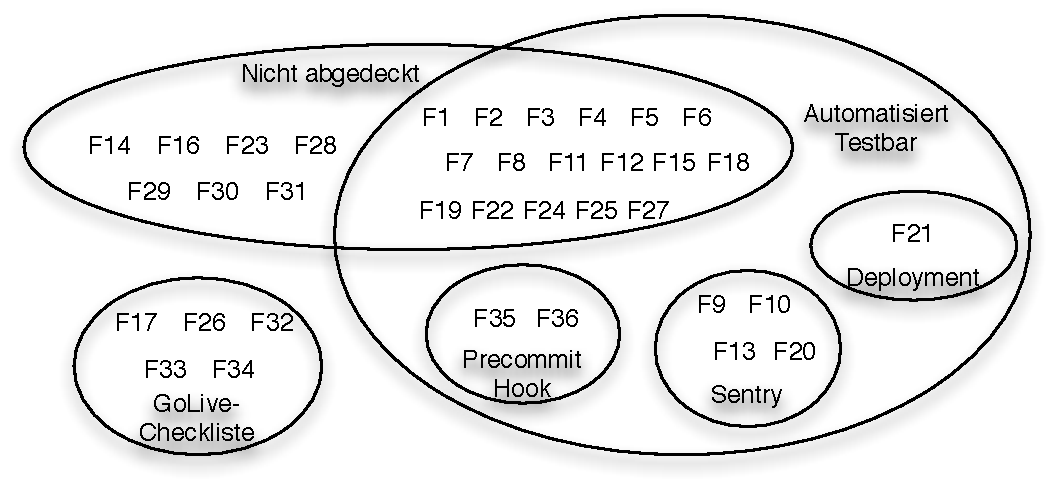
\includegraphics[width=1\textwidth]{images/abdeckung.pdf}
\caption{Übersicht Fehlerszenarios}
\label{fig:uebersicht_fehlerszenarios}
\end{figure}

\section{Fehlerszenarios welche abgedeckt werden müssen}
\label{sec:fehlerszenarios_welche_abgedeckt_werden_müssen}
Die Fehlerszenarios welche nicht durch die bereits vorhandenen Systeme abgedeckt werden, sollen gemäss Aufgabenstellung in automatisiert und manuell testbar unterteilt werden. Als manuell testbar ist ein Szenario dann, wenn es durch eine Software geprüft werden kann. So sind zum Beispiel Rechtschreibfehler nicht automatisiert Prüfbar, da zur Zeit keine Rechtschreibprüfung vollautomatisiert arbeiten kann. Es ist immer zusätzlich ein Mensch nötig welcher entscheiden muss, ob zum Beispiel ein Wort ein Name ist und daher nicht im Wörterbuch zu finden ist.

\subsubsection{Automatisiert testbar}
\label{ssub:automatisiert_testbar}

\ref{f:zertifikatausgelaufen} \fzertifikatausgelaufen, \ref{f:zertifikatungultig} \fzertifikatungultig, \ref{f:sslnichterzwungen} \fsslnichterzwungen, \ref{f:externeassetsohnessl} \fexterneassetsohnessl, \ref{f:domainausgelaufen} \fdomainausgelaufen, \ref{f:dnsservernichtverfuegbar} \fdnsservernichtverfuegbar, \ref{f:dnseintragfehlerhaft} \fdnseintragfehlerhaft, \ref{f:spfeintragfehlerhaft} \fspfeintragfehlerhaft, \ref{f:deprecatedlibraries} \fdeprecatedlibraries, \ref{f:unittestfehler} \funittestfehler, \ref{f:debugmodus} \fdebugmodus, \ref{f:datenbankquerieslaufenlangsam} \fdatenbankquerieslaufenlangsam, \ref{f:applikationlaeuftlangsam} \fapplikationlaeuftlangsam, \ref{f:seitelaedtzulangsam} \fseitelaedtzulangsam, \ref{f:assetsfehlen} \fassetsfehlen, \ref{f:externeabhaengigkeiten} \fassetsfehlen, \ref{f:seiteenthaelttotelinks} \fseiteenthaelttotelinks

\subsubsection{Manuell testbar}
\label{ssub:manuel_testbar}

\ref{f:missverhalten} \fmissverhalten, \ref{f:abhaengigkeitenmitsicherheitsluecken} \fabhaengigkeitenmitsicherheitsluecken, \ref{f:browserspezifischeprobleme} \fbrowserspezifischeprobleme, \ref{f:rechtschreibefehler} \frechtschreibefehler, \ref{f:falschaufbereitetebilder} \ffalschaufbereitetebilder, \ref{f:designverletzt} \fdesignverletzt, \ref{f:fehlmanipulationdurchdenkunden} \ffehlmanipulationdurchdenkunden

  
  \chapter{Anforderungsanalyse}
  \label{cha:anforderungsanalyse}
  %!TEX root = ../index.tex

\newcounter{anumber} \setcounter{anumber}{0}
\renewcommand\theanumber{A\arabic{anumber}}
\newcommand{\newanumber}[3]%
{%
\midrule%
\refstepcounter{anumber}\label{a:#1}%
\theanumber & #2 & #3 \\
}


\section{Systemkontext}
\label{sec:systemkontext}
Der Systemkontext für Programme, welche die Qualität von Webprojekten überprüfen und sicherstellen, ist für alle Programme derselbe. In diesem Systemkontext sind bereits mehrere Programme und Systeme vorhanden. Die neu einzuführenden Systeme sollen wo auch immer möglich mit den bereits vorhandenen zusammenarbeiten.

\subsection{allink.planer}
\label{sub:allink_planer}
Der allink.planer ist ein Programm welches in der allink entwickelt wurde. Im allink.planer sind zur Zeit diverse Funktionen implementiert. Die Funktionalitäten im allink.planer, welche den für diese Arbeit relevant sind, werden im Folgenden kurz erklärt. Weiterhin sind im allink.planer vor allem Funktionalitäten für die Auswertung von Projekten implementiert, sowie auch ein Rechnungs und Offertensystem.

\subsubsection{Hosting Tracking}
\label{ssub:hosting_tracking}
Um die jährlichen Hostingrechnungen zu automatisieren, wurde in den allink.planer ein Programm eingebaut, welches sämtliche Produktivserver der allink täglich überprüft, alle darauf existierenden Webprojekte sammelt und ein Verzeichnis dieser aktuell hält. In diesem System sind alle für diese Arbeit relevanten Webprojekte verzeichnet. Wo möglich sollen neue Systeme mit diesem Verzeichnis arbeiten, damit neue Webprojekte nicht von Hand erfasst werden müssen.

\subsection{Produktivsysteme}
\label{sub:produktivsysteme}
Mit Produktivsystemen sind die Server gemeint, auf welchen die Webapplikationen, welche in der allink entwickelt werden, gehostet sind. Im Normalfall handelt es sich hier um virtuelle Server, welche von der Firma Nine Internet Solutions AG betrieben und unterhalten werden. Dadurch ist die Verantwortung für den Betrieb der Server nicht bei der allink und die Software-Entwickler können sich auf die Applikation konzentrieren. Um den Betrieb der Server zu kontrollieren, setzt Nine Internet Solutions eine Monitoring-Software ein. Diese Software ist jedoch ausserhalb des Systemkontext und sollte daher keinen Einfluss auf diese Arbeit haben.

\section{Stakeholder}
\label{sec:stakeholder}


\subsection{Programmierer}
\label{sub:programmierer}
Die Programmierer in der allink setzen meist mehrere Projekte pro Person im Monat um. Vor allem bei kleineren Projekten, kann es vorkommen, dass nach wenigen Tagen das Projekt abgeschlossen ist. Da viele Webseiten nach einiger Zeit kleine Aktualisierungen benötigen, ist es wichtig, dass alle Projekte möglichst die selbe Projektstruktur haben. Die Programmierer erwarten daher, dass die neuen Systeme zur Erhaltung der Qualität gut in das bestehende Setup integriert werden können.

\subsection{Projektleitung}
\label{sub:projektleitung}
Die Projektleitung besteht in der allink hauptsächlich aus den vier Teilhabern. Diese erwarten, dass sie durch die neuen Systeme keine zusätzlichen Aufgaben erhalten. Da sich erhöhte Qualität bei Kunden schlecht als Mehrwert verkaufen lässt, erwartet die Projektleitung, dass sich der Mehraufwand, welcher für jedes Projekt anfällt, durch die Ersparnisse durch verfrühtes Erkennen von Problemen lohnt. Es sollen jedoch in Zukunft Fehler und Probleme wo möglich erkannt werden, bevor der Kunde diese entdeckt.

\subsection{Geschäftsleitung}
\label{sub:geschäftsleitung}
Die Geschäftsleitung erwartet, dass die Kosten, welche mit den neuen Systemen entstehen, in einem angemessenen Rahmen bleiben.

\subsection{Kunde}
\label{sub:kunde}
Kunden der allink erwarten, dass ihre Webprojekte möglichst ohne Fehler laufen und dauernd verfügbar sind. Da viele Kunden kein oder nur wenig Wissen im Bereich der Informatik haben, können sie teils nur schwer nachvollziehen, warum ein System auch nach dem die Programmierarbeiten abgeschlossen, sind weiter betreut werden muss. Sie erwarten, dass trotz ändernden Bedingungen durch neue Browser ihre Webseite auf den häufigsten Browsern richtig dargestellt wird und falls ein Problem auftritt, dieses möglichst schnell behoben wird.

\subsection{Hostingprovider}
\label{sub:hosting_provider}
Die Nine Internet Solutions AG ist Hostingprovider für alle Produktivsysteme der allink. Nine will weiterhin eine klare Trennung der Zuständigkeit wie dies bis anhin der Fall war. Es sollen zudem keine neuen Aufgaben für Nine entstehen.

\section{Anforderungen}
\label{sec:anforderungen}

Für alle Anforderungen wird von 100 Webapplikationen verteilt auf 5 Server ausgegangen.

\begin{longtable}{l>{\raggedright}p{4cm} p{8cm}}
    \toprule \textbf{Nr.} & \textbf{Quelle} & \textbf{Beschreibung} \\
    \newanumber{einfach_implementierbar}{Programmierer}{Sämtliche zusätzliche Systeme sollen einfach in den allink Programmierprozess integrierbar sein.}
    \newanumber{kosten}{Geschäftsleitung}{Für die bestehenden Produktivsysteme sollen die Kosten für externe Systeme nicht CHF 6000 pro Jahr übersteigen.}
    \newanumber{aufwand}{Projektleitung}{Es soll auf Projektebene kein Mehraufwand entstehen.}
    \newanumber{sicherheit}{Programmierer}{Alle externen Tools welche Benutzerdaten benötigen sollen über eine sichere Verbindung verfügbar sein.}
    \newanumber{hosting}{Hostingprovider}{Es sollen keine neuen Zuständigkeiten und Aufgaben für den Hostingprovider entstehen.}
    \bottomrule
    \caption[Anforderungen]{Anforderungen}
    \label{tab:anforderungen}
\end{longtable}

Zusätzlich zu diesen Anforderungen, sollen alle eingesetzten Tools zusammen mit den bestehenden Mitteln und den übrigen Neuerungen den gesamten Fehlerkatalog aus Kapitel~\ref{cha:fehlerkatalog} abdecken. 

  
  \chapter{Evaluation}
  \label{cha:evaluation}
  %!TEX root = ../index.tex

Der Markt für Tools welche die Qualitätssicherung von Softwareprojekten unterstützt ist ziemlich gross. Anhand der Fehlerszenarios welche nicht durch ein bestehendes System abgedeckt werden können die zu evaluierenden Tools stark eingegrenzt werden. So ist zum Beispiel kein Tool welches den Programmcode mittels statischer Analyse bewertet notwendig, da eine solche Analyse bereits in \ref{b:precommithook} durchgeführt wird. Um die offenen Fehlerszenarios abzudecken wurde in den Bereichen Monitoring und Continuous Integration nach geeigneten Lösungen gesucht.

\section{Monitoring}
\label{sec:monitoring_evaluation}
Eine grosse Zahl an Produkten existiert mit welchen man eine Webapplikation in regelmässigen Abständen überprüfen kann. Viele Produkte greifen nur von ausserhalb auf die Webapplikaiton und benachrichtigen falls diese nicht wie zuvor definiert verfügbar sein sollte. Einige Tools setzen jedoch bereits in der Applikation an und können da auch die Zeit welche eine Applikation für eine Anfrage braucht, oder die Menge und der Zeitbedarf von Datenbankabfragen messen. Ein Real User Monitoring welches direkt im Browser des Benutzers läuft, berücksichtigt zusätzlich die Geschwindigkeit der Internet-Verbindung und den verwendeten Browser.

\ref{f:zertifikatausgelaufen}, \ref{f:zertifikatungultig}, \ref{f:sslnichterzwungen}, \ref{f:externeassetsohnessl}, \ref{f:domainausgelaufen}, \ref{f:dnsservernichtverfuegbar}, \ref{f:dnseintragfehlerhaft}, \ref{f:spfeintragfehlerhaft}, \ref{f:deprecatedlibrarys}, \ref{f:debugmodus}, \ref{f:datenbankquerieslaufenlangsam}, \ref{f:applikationlaeuftlangsam}, \ref{f:seitelaedtzulangsam}, \ref{f:assetsfehlen}, \ref{f:externeabhaengigkeiten}, \ref{f:seiteenthaelttotelinks}

\subsection{Marktanalyse}
\label{sub:marktanalyse}

\subsubsection{Sillalive}
\label{ssub:sillalive}

\begin{table}[h!]
  \centering
  \begin{tabular}{p{5cm} p{7cm}}
  \toprule
    Webseite & \url{https://stillalive.com/}\\
  \hline
    Preisplan & Startup\\
  \hline
    Preismodell & 15\$ pro Seite pro Monat pro Webseite\\
  \hline
    Jährliche Kosten & 18000\$\\
  \hline
    Erfüllte Anforderungen & \ref{a:einfach_implementierbar}, \ref{a:aufwand}, \ref{a:sicherheit}, \ref{a:hosting}\\
  \hline
    Abgedeckte Fehlerszenarios & Nicht evaluiert\\
  \bottomrule
  \end{tabular}
  \caption{Stillalive}
  \label{tab:stillalive}
\end{table}

Scheidet schon durch die hohen Kosten aus. Ist eher für Firmen welche eine einzige Webapplikation überwachen wollen geeignet.

\subsubsection{Newrelic}
\label{ssub:newrelic}

\begin{table}[h!]
  \centering
  \begin{tabular}{p{5cm} p{7cm}}
  \toprule
    Webseite & \url{https://newrelic.com/}\\
  \hline
    Preisplan & Standard\\
  \hline
    Preismodell & 24\$ pro Monat pro Server\\
  \hline
    Jährliche Kosten & 1440\$\\
  \hline
    Erfüllte Anforderungen & \ref{a:einfach_implementierbar}, \ref{a:kosten}, \ref{a:aufwand}, \ref{a:sicherheit}, \ref{a:hosting}\\
  \hline
    Abgedeckte Fehlerszenarios & \ref{f:domainausgelaufen}, \ref{f:dnsservernichtverfuegbar}, \ref{f:dnseintragfehlerhaft}, \ref{f:applikationlaeuftlangsam}, \ref{f:seitelaedtzulangsam}\\
  \bottomrule
  \end{tabular}
  \caption{New Relic Standard}
  \label{tab:new_relic_standard}
\end{table}

\begin{table}[h!]
  \centering
  \begin{tabular}{p{5cm} p{7cm}}
  \toprule
    Webseite & \url{https://newrelic.com/}\\
  \hline
    Preisplan & Enterprise\\
  \hline
    Preismodell & 149\$ pro Monat pro Server\\
  \hline
    Jährliche Kosten & 8940\$\\
  \hline
    Erfüllte Anforderungen & \ref{a:einfach_implementierbar}, \ref{a:kosten}, \ref{a:aufwand}, \ref{a:sicherheit}, \ref{a:hosting}\\
  \hline
    Abgedeckte Fehlerszenarios & \ref{f:externeassetsohnessl}, \ref{f:domainausgelaufen}, \ref{f:dnsservernichtverfuegbar}, \ref{f:dnseintragfehlerhaft}, \ref{f:datenbankquerieslaufenlangsam}, \ref{f:applikationlaeuftlangsam}, \ref{f:seitelaedtzulangsam}, \ref{f:assetsfehlen}, \ref{f:externeabhaengigkeiten}\\
  \bottomrule
  \end{tabular}
  \caption{New Relic Enterprise}
  \label{tab:new_relic_enterprise}
\end{table}

New Relic kann eine Webapplikation mit einem Statistischen Profiler durchleuchten und somit einen Einblick in die laufende Applikation gewähren. Zusätzlich bietet es zentrales Errorreporting, Real User Monitoring und viele kleinere Tools.

\subsubsection{Pingdom}
\label{ssub:pingdom}

\begin{table}[h!]
  \centering
  \begin{tabular}{p{5cm} p{7cm}}
  \toprule
    Webseite & \url{https://www.pingdom.com/}\\
  \hline
    Preisplan & Team\\
  \hline
    Preismodell & 495\$ pro Monat\\
  \hline
    Jährliche Kosten & 5940\$\\
  \hline
    Erfüllte Anforderungen & \ref{a:einfach_implementierbar}, \ref{a:kosten}, \ref{a:aufwand}, \ref{a:sicherheit}, \ref{a:hosting}\\
  \hline
    Abgedeckte Fehlerszenarios & \ref{f:zertifikatausgelaufen}, \ref{f:zertifikatungultig}, \ref{f:domainausgelaufen}, \ref{f:dnsservernichtverfuegbar}, \ref{f:dnseintragfehlerhaft}, \ref{f:seitelaedtzulangsam}, \ref{f:assetsfehlen}, \ref{f:externeabhaengigkeiten}, \ref{f:seiteenthaelttotelinks}\\
  \bottomrule
  \end{tabular}
  \caption{Pingdom}
  \label{tab:pingdom}
\end{table}

Für Firmen welche eine einzige Webseite oder Webapplikation entwickeln bietet sich Pingdom an. Es bietet neben einer Push Notification fähigen iOS Applikation auch Real User Monitoring.

\subsubsection{Status Cake}
\label{ssub:status_cake}

\begin{table}[h!]
  \centering
  \begin{tabular}{p{5cm} p{7cm}}
  \toprule
    Webseite & \url{https://www.statuscake.com/}\\
  \hline
    Preisplan & Superior\\
  \hline
    Preismodell & 6.49£ pro Monat\\
  \hline
    Jährliche Kosten & 78£\\
  \hline
    Erfüllte Anforderungen & \ref{a:einfach_implementierbar}, \ref{a:kosten}, \ref{a:aufwand}, \ref{a:sicherheit}, \ref{a:hosting}\\
  \hline
    Abgedeckte Fehlerszenarios & \ref{f:zertifikatausgelaufen}, \ref{f:zertifikatungultig}, \ref{f:domainausgelaufen}, \ref{f:dnsservernichtverfuegbar}, \ref{f:dnseintragfehlerhaft}, \ref{f:seitelaedtzulangsam}, \ref{f:seiteenthaelttotelinks}\\
  \bottomrule
  \end{tabular}
  \caption{Status Cake}
  \label{tab:status_cake}
\end{table}

Status Cake bietet ziemlich viel wenn man den niedrigen Preis bedenkt. Im Preisplan Superior ist ein automatisiertes einfügen von neuen Webseiten welche zu testen sind möglich.

\subsubsection{Web on Duty}
\label{ssub:web_on_duty}

\begin{table}[h!]
  \centering
  \begin{tabular}{p{5cm} p{7cm}}
  \toprule
    Webseite & \url{https://webonduty.com/}\\
  \hline
    Preisplan & Test jede Stunde\\
  \hline
    Preismodell & 36£ pro Monat\\
  \hline
    Jährliche Kosten & 432£\\
  \hline
    Erfüllte Anforderungen & \ref{a:einfach_implementierbar}, \ref{a:kosten}, \ref{a:aufwand}, \ref{a:sicherheit}, \ref{a:hosting}\\
  \hline
    Abgedeckte Fehlerszenarios & \ref{f:domainausgelaufen}, \ref{f:dnsservernichtverfuegbar}, \ref{f:dnseintragfehlerhaft}\\
  \bottomrule
  \end{tabular}
  \caption{Web on Duty}
  \label{tab:web_on_duty}
\end{table}

Web on Duty kann keine ungültige oder abgelaufene SSL-Zertifikate detektieren. Lässt man es eine Webseite mit einem ungültigen Zertifikat überprüfen meldet es keinen Fehler.

\subsection{Entscheid}
\label{sub:entscheid_monitoring}
Es lassen sich grundsätzlich alle automatisiert Testbaren Fehlerszenarios mit Eigenentwicklungen abdecken, der Aufwand um dies zu erreichen ist aber nicht verhältnismässig. Da nicht ein Produkt evaluiert wird, sondern eine Kombination aus mehreren, gibt es zu viele einzelne Kombinationen um auf jede mögliche einzugehen. Die möglichen Kombinationen wurden als mehrkriterieles Optimierungproblem angegangen. So wurden Lösungen welche von besseren Lösungen dominiert wurden ausgeschlossen und in der daraus entstehenden Lösungsmenge zwei mögliche Lösungen betrachtet.


Mit NewRelic standard und Status Cake bleiben folgende Punkte noch offen:

\ref{f:sslnichterzwungen}, \ref{f:externeassetsohnessl}, \ref{f:spfeintragfehlerhaft}, \ref{f:deprecatedlibrarys}, \ref{f:debugmodus}, \ref{f:datenbankquerieslaufenlangsam}, \ref{f:applikationlaeuftlangsam}, \ref{f:assetsfehlen}, \ref{f:externeabhaengigkeiten}

Mit NewRelic enterprise und Status Cake und bleiben folgende Punkte noch offen:

\ref{f:sslnichterzwungen}, \ref{f:spfeintragfehlerhaft}, \ref{f:deprecatedlibrarys}, \ref{f:debugmodus}

\section{Continuous Integration}
\label{sec:continuous_integration_evaluation}
Um das Fehlerszenario \ref{f:unittestfehler} automatisiert abzudecken wird ein System benötigt welches jeweils den aktuellen Programmcode automatisch überprüft. Es gibt diverse Continous Integration Lösungen welche sich für diese Aufgabe eignen. Bei Django Projekten sind die beiden CI Systeme Travis und Jenkins am weitesten verbreitet. Weiterhin wurde auch das in Python geschriebe Buildbot evaluiert.

\begin{enumerate}
  \item https://travis-ci.org
  \item http://buildbot.net
  \item http://jenkins-ci.org
\end{enumerate}

\subsection{Anforderungen}
\label{sub:anforderungen}
Da die allink nicht wie viele andere Benutzer eines CI Systems ein einziges Produkt entwickelt, sondern viele einzelne Projekte betreibt, ist nicht jedes System geeignet. Weiterhin soll auch hier gemäss Anforderung \ref{a:einfach_implementierbar} möglichst kein zusätzlicher Aufwand für jedes einzelne Projekt entstehen.

\subsection{Entscheid}
\label{sub:entscheid_ci}
Da die allink keinen eigenen CI Server betreiben will, kommen nur Systeme in Frage, welche auch als Service angeboten werden. Daher is Buildbot basiertes System für allink nicht geeignet.

Zu den zwei verbleibenden Systemen wurde jeweils ein günstiger Anbieter welcher dieses Produkt als Service anbietet gesucht um sicherzustellen, dass ein solcher vorhanden ist. So wurde für Travis welches Open Source ist, vom Hersteller auch für Business-Kunden angeboten. Dieser Service findet sich unter \url{https://travis-ci.com} und ist zur Zeit nur mit einer Einladung verfügbar. Jenkins ist bei \url{http://www.cloudbees.com/} als Service erhältlich.
 
Da in der allink zum Teil schon Erfahrungen mit dem Umgang mit Travis bestehen und dieser Service Anforderungen erfüllt, wurde in Absprache mit der Informatik Leitung in die Entscheidung gefällt, Travis zu verwenden.

\section{Neue Systeme}
\label{sec:neue_systeme}

\makeatletter
\newcounter{lnumber} \setcounter{lnumber}{0}
\renewcommand\thelnumber{L\arabic{lnumber}}
\newcommand{\newlnumber}[3]%
{%
\midrule%
\refstepcounter{lnumber}%
\expandafter\xdef\csname l#2\endcsname {#1}%
\thelnumber\label{l:#2} & #1 & #3 \\
}
\makeatother

\begin{longtable}{l>{\raggedright}p{5cm} p{5cm}}
    \toprule \textbf{Nr.} & \textbf{Bezeichnung} & \textbf{Preismodell} \\
    \newlnumber{New Relic}{newrelic}{Enterprise}
    \newlnumber{StatusCake}{statuscake}{Superior}
    \newlnumber{Travis}{travis}{Enterprise}
    \bottomrule
    \caption[Neue Systeme]{Neue Systeme}
    \label{tab:neue_systeme}
\end{longtable}


  \chapter{Proof of Concept}
  \label{cha:proof_of_concept}
  %!TEX root = ../index.tex

\section{Deprecated Libraries}
\label{sec:deprecated_libraries}
Der Punkt \ref{f:deprecatedlibraries} ist theoretisch automatisch testbar. Man könnte dem Precommit Hook entsprechende Logik einbauen. In der Praxis ist es jedoch nicht sinnvoll eine Webseite als Fehlerhaft zu markieren nur weil es teile einer Library braucht welche in der nächsten Version nicht mehr vorhanden sind. Darum wurde zusammen mit der Informatikleitung entschieden, dass dieses Fehlerszenario beim Abschluss eines Projektes von Hand geprüft werden soll. Der Go-Live Checkliste wurde ein Punkt hinzugefügt um diesen Punkt abzudecken.

\section{Wiederkehrende manuelle Tests}
\label{sec:wiederkehrende_manuelle_tests}
Zusätzlich zu der bestehenden Go-Live Checkliste wurde eine Checkliste erstellt, welche bei Webprojekten nach dem Go-Live regelmässig durchgegangen wird. Diese Checkliste ist in Tabelle~\ref{tab:recuring_checklist} ersichtlich.

\makeatletter
\newcounter{tnumber} \setcounter{tnumber}{0}
\renewcommand\thetnumber{T\arabic{tnumber}}
\newcommand{\newtnumber}[3]%
{%
\midrule%
\refstepcounter{tnumber}%
\expandafter\xdef\csname t#2\endcsname {#1}%
\thetnumber\label{t:#2} & #1 & #3 \\
}
\makeatother

\begin{table}[ht]
  \centering
  \begin{tabular}{l>{\raggedright} p{10cm} p{2cm}}
    \toprule \textbf{Nr.} & \textbf{Test} & \textbf{Abgedeckte Fehlerszenarios} \\
    \newtnumber{Funktioniert die Webseite erwartungsgemäss? Ist offensichtliches Fehlverhalten vorhanden?}{missverhalten}{\ref{f:missverhalten}}
    \newtnumber{Sind die verwendeten Versionen von Django, feincms etc. noch aktuell?}{abhaengigkeitenmitsicherheitsluecken}{\ref{f:abhaengigkeitenmitsicherheitsluecken}}
    \newtnumber{Funktioniert die Seite in den aktuellen Versionen von Safari, Firefox, Chrome und IE?}{browserspezifischeprobleme}{\ref{f:browserspezifischeprobleme}}
    \newtnumber{Sind auf der Startseite und den Landingpages offensichtliche Rechtschreibefehler?}{rechtschreibefehler}{\ref{f:rechtschreibefehler}}
    \newtnumber{Sind die verwendeten Bilder richtig aufbereitet?}{falschaufbereitetebilder}{\ref{f:falschaufbereitetebilder}}
    \newtnumber{Wurde das Design offensichtlich verletzt?}{designverletzt}{\ref{f:designverletzt}}
    \bottomrule
  \end{tabular}
  \caption{Checkliste für wiederkehrende Überprüfungen}
  \label{tab:recuring_checklist}
\end{table}

\section{Continuous Integration}
\label{sec:continuous_integration_proof_of_concept}
Da Travis für Unternehmen zur Zeit noch nicht frei verfügbar ist, wurde Travis angeschrieben und unsere Situation geschildert. Darauf erhielt allink die benötigte Einladung um Travis zu benutzen.
Um Travis in den bestehenden Projekt Workflow zu integrieren, wurde im der Basiscodebase welche für jedes Django Softwareprojekt verwendet wurde ein .travis.yml erstellt, welches die genaue Testkonfiguration und den Ablauf beinhaltet.

\section{Monitoring}
\label{sec:monitoring_proof_of_concept}
Um alles Webprojekte automatisiert zu überprüfen wurden zwei neue Systeme eingeführt und ein bereits bestehendes System erweitert.

\subsection{Status Cake}
\label{sub:status_cake}
Als erstes neues System wurde Status Cake für alle Webprojekte eingeführt. Damit wird im Minutentakt überprüft, ob die Seiten noch erreichbar sind und ob mit den SSL Zertifikaten alles in Ordnung ist. Zudem werden einmal täglich alle Webseiten nach toten Links durchsucht.

Damit die Tests in Status Cake nicht von Hand nachgetragen werden müssen, wurde der allink.planer so erweitert, dass er Webprojekte automatisch beim Erfassen direkt zu Status Cake hinzufügt.

\begin{figure}[ht]
\centering
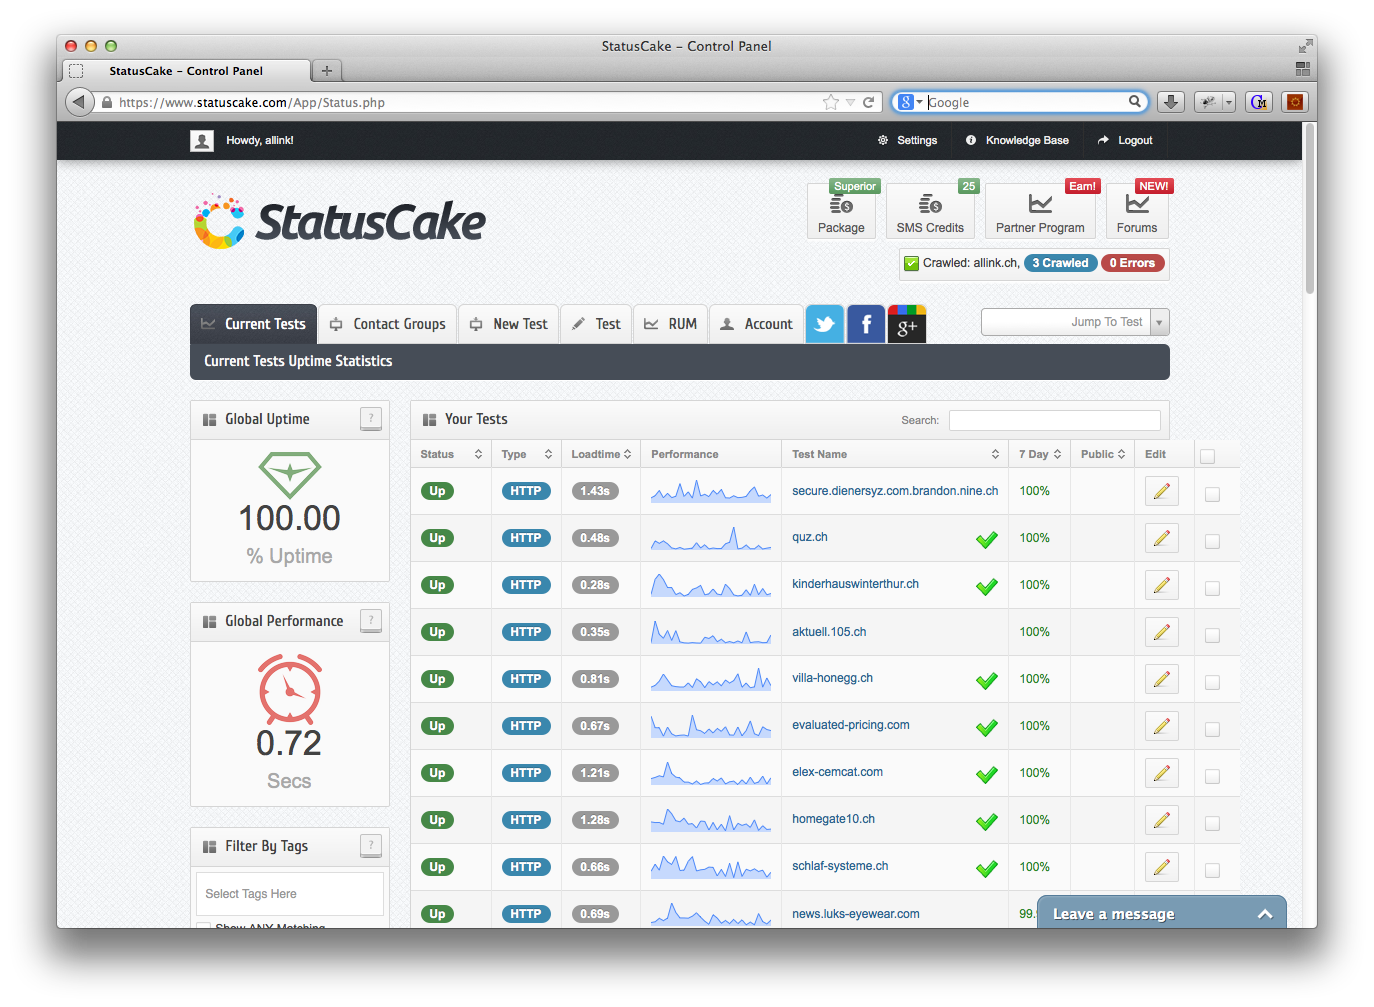
\includegraphics[width=1\textwidth]{images/status_cake.png}
\caption{Status Cake Übersicht}
\label{fig:status_cake}
\end{figure}


\subsection{New Relic}
\label{sub:new_relic}
Weiterhin wurde für einige Webprojekte New Relic eingeführt. Ein bestehendes Projekt mit New Relic auszurüsten ist einiges Aufwendiger, als es mit Status Cake auszurüsten. Für die Integration von New Relic müssen Änderungen am Programmcode vorgenommen werden. Dies ist bei neuen Projekten kein Problem, da für neue Projekte ein Template verwendet wird.

Das Preismodel von New Relic berechnet die Kosten anhand der Anzahl Server welche verwendet werden. Da in der allink demnächst ein grosser Teil der Produktiven Systeme ersetzt werden und danach auch weniger Server eingesetzt werden, wird mit dem Einsatz von New Relic für alle Projekte gewartet, bis diese Umstellung erfolgt ist. Bis dahin werden nur zwei Projekte mit New Relic ausgestattet.

New Relic bietet unter anderem eine Mobile Applikation welche die wichtigsten Daten einer Webseite anzeigen kann. Zudem gibt es für jedes Projekt ein Dashboard wie in Abbildung~\ref{fig:new_relic_dashboard} gezeigt wird, auf welchem man Probleme jeder Art schnell erkennen kann.

\begin{figure}[ht]
\centering
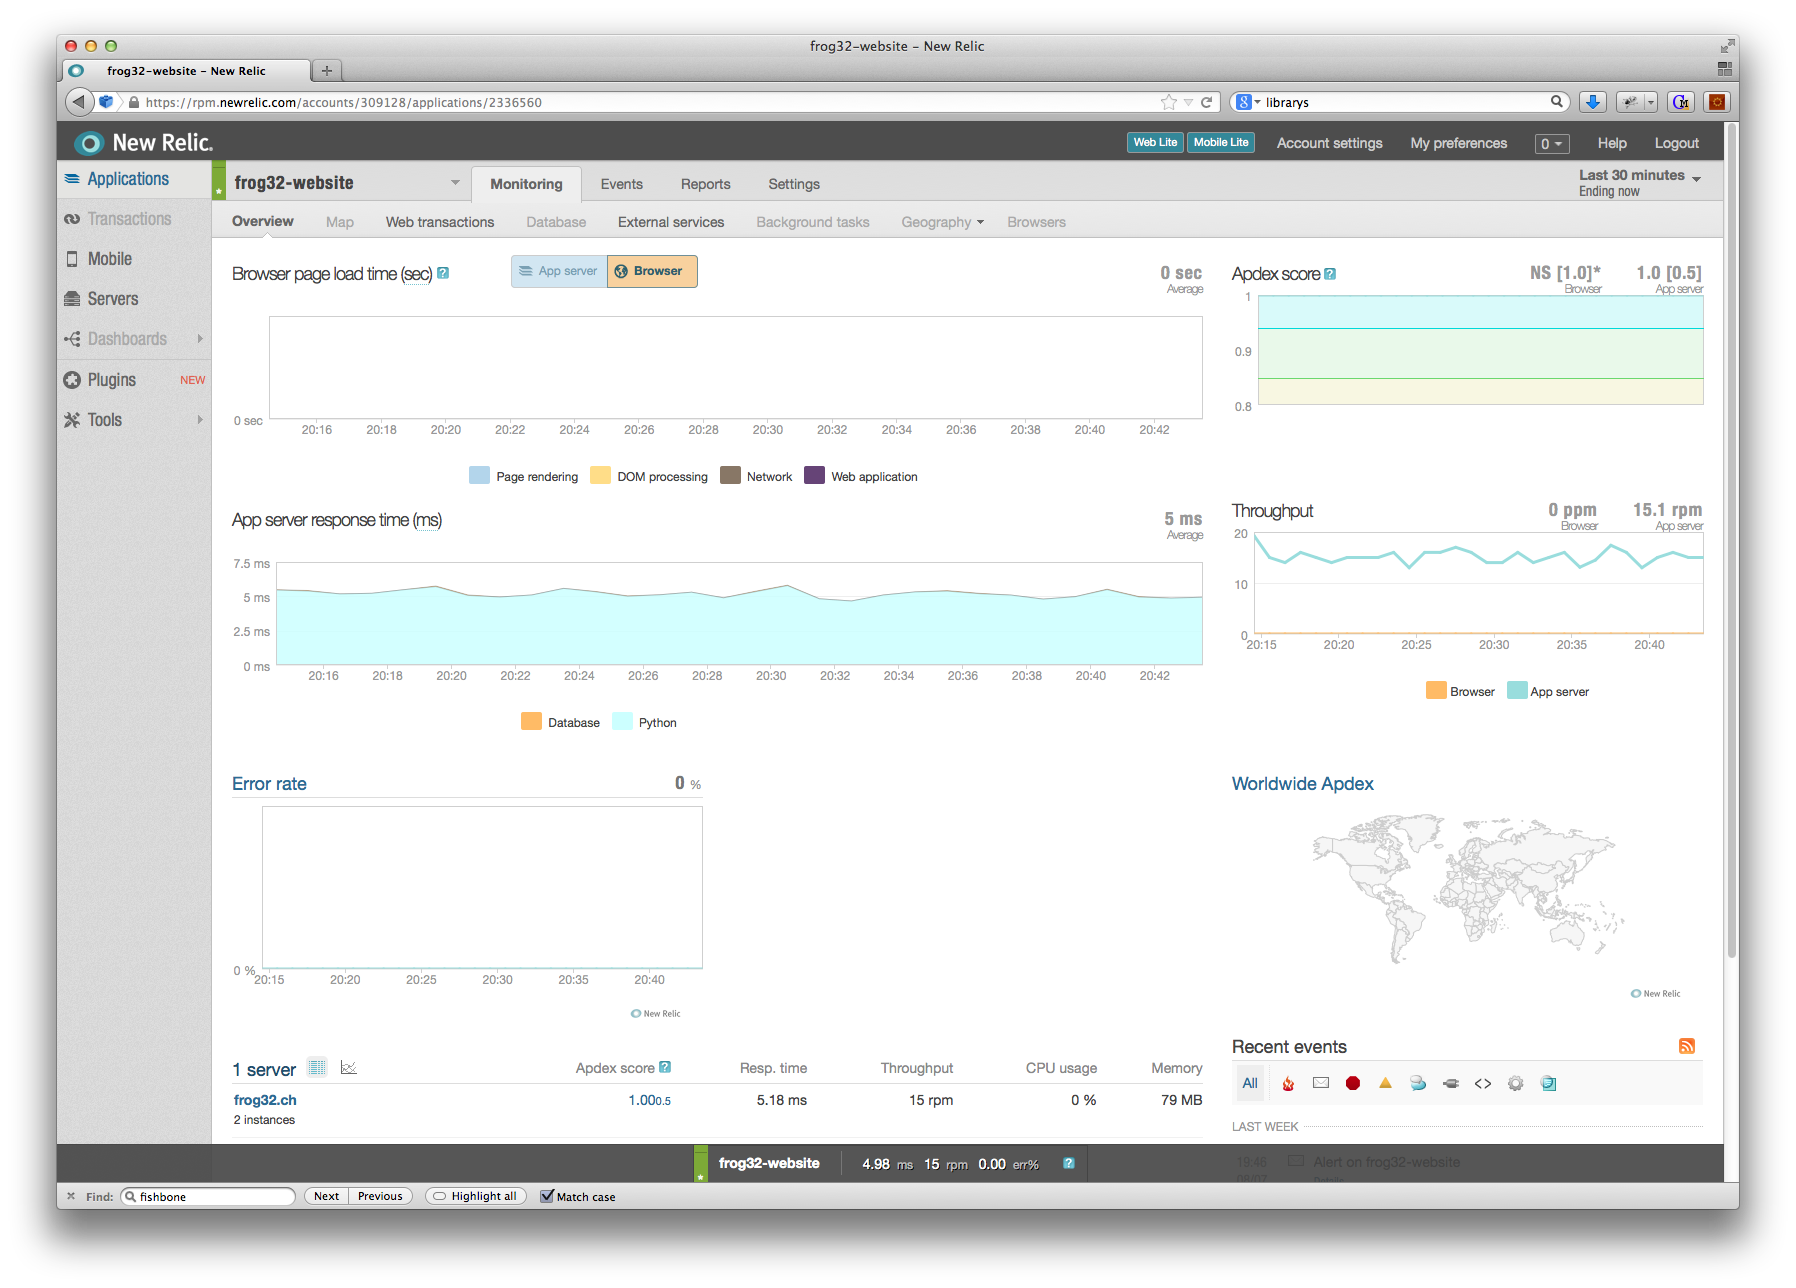
\includegraphics[width=1\textwidth]{images/new_relic.png}
\caption{New Relic Dashboard}
\label{fig:new_relic_dashboard}
\end{figure}


\subsection{allink.planer}
\label{sub:proof_allink_planer}
Der allink.planer wurde wo erweitert, dass er die Fehlerszenarios \ref{f:sslnichterzwungen}, \ref{f:spfeintragfehlerhaft} und \ref{f:debugmodus} abdecken kann. Dies sind alles Fehlerszenarios welche ohne Probleme von ausserhalb eines Webprojektes überprüfbar sind. Weiterhin wurde der allink.planer so erweitert, dass er fähig ist die Versionen von verwendeten Python Paketen jedes Projektes auszulesen. Damit lässt sich im Falle, dass eine Sicherheitslücke bekannt wird schnell feststellen in welchen Projekten die betroffenen Softwareversionen eingesetzt wurden. Damit wird das manuelle Überprüfen von Fehlerszenario \ref{f:abhaengigkeitenmitsicherheitsluecken} massiv vereinfacht.

\section{Auswirkungen}
\label{sec:auswirkungen}
Mit all den neuen Tools wurde auch die Menge an E-Mails welche jeder Entwickler täglich erhält stetig grösser. So versendet zum Beispiel Status Cake jedes mal ein E-Mail, wenn eine zu überwachende Seite nicht mehr erreichbar ist. Dies führte dazu, dass die meisten Entwickler diese E-Mails mittels Regeln direkt in eigene Ordner verschieben lassen. So fällt es nicht mehr direkt auf, wenn eine Webseite nicht mehr erreichbar ist, da das E-Mail welches darauf hinweisen soll, automatisch aus dem Posteingang entfernt wird und in einen eigenen Ordner bewegt wird welche für solche Benachrichtigungen vorgesehen ist. Dadurch bleibt übrigen E-Mails im Posteingang mehr Aufmerksamkeit, jedoch kann es vorkommen, dass ein schwerwiegender Fehler über einen Tag nicht bemerkt wird.

E-Mails welche von Sentry versendet werden teilweise ignoriert, da die Fehler auch in Sentry selber noch angezeigt werden. Leider haben sich zuwenig Entwickler regelmässig die Fehlerliste in Sentry oder die Status Seite von Travis angesehen. Dies führte dazu, dass die gewünschte Wirkung nicht ganz erzielt wurde.

\subsection{Status Monitor}
\label{sub:status_monitor}
Um sicherzustellen, dass Fehler auch wahrgenommen werden, wurde als Zusatz zu den bereits eingeführten Systemen ein Status Monitor eingeführt. Ein Bildschirm welcher vom Arbeitsplatz sämtlicher Entwickler sichtbar ist wurde mit einem am VESA Mount des Displays befestigten Computer ausgestattet. Dabei wurde darauf geachtet, dass der Computer genügend Leistung hat um in einem Webbrowser eine Javascript Applikation ohne Probleme zu betreiben und dass der Stromverbrauch des Computers deutlich unter dem Nivea eines Arbeitsplatzcomputers ist, da dieser Computer ununterbrochen laufen wird.

\subsubsection{Software}
\label{ssub:software}
Das Backend der Software welche die Daten aus verschiedenen Quellen aggregiert wurde mit dem Twisted\footnote{\url{http://twistedmatrix.com/}} Framework in der Programmiersprache Python erstellt. Das Interface welches im Webbrowser läuft wurde als Backbone\footnote{\url{http://backbonejs.org/}} Applikation realisiert um auch Clientseitig eine Templateengine zu haben.

Das Frontend kommuniziert mit dem Backend über einen Websocket. Damit lassen sich Daten asynchron zwischen Frontend und Backend austauschen. Die ganze Software wurde modular aufgebaut damit sich in Zukunft weitere Syteme daran anbinden lassen.

\begin{figure}[ht]
\centering
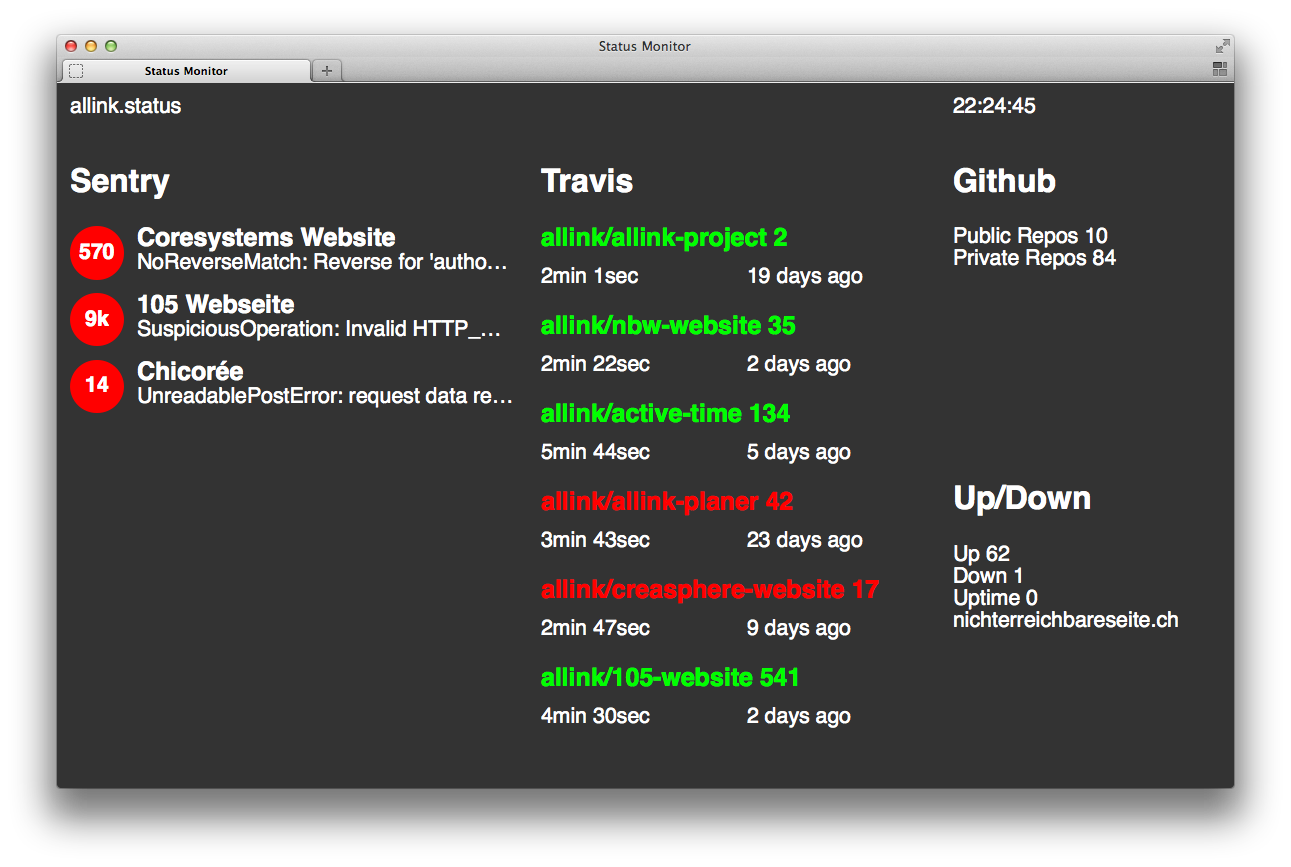
\includegraphics[width=1\textwidth]{images/status_monitor.png}
\caption{Status Monitor}
\label{fig:status_monitor}
\end{figure}

  
  \chapter{Fazit}
  \label{cha:fazit}
  
  \appendix  
  \listoffigures
  \listoftables
  \lstlistoflistings
  
  \glsaddall
  \printglossaries
  
  \nocite{*}
  \bibliographystyle{alphadin}
  \bibliography{cite}
\end{document}
